\section{9649 JC2 Preliminary Examination Paper 2}

\begin{problem}
    The largest positive root, $\a$, of $5x - x^3 = \e^{-x}$ falls in the interval $N \leq x \leq N + 1$, where $N$ is an integer.

    \begin{enumerate}
        \item By sketching the graph of $y = 5x - x^3$ and $y = \e^{-x}$, show that $N = 2$.
        \item Use linear interpolation once on the interval $[N, N+1]$, with $f(x) = 5x - x^3 - \e^{-x}$ to find an approximation to $\a$, giving your answer to 5 decimal places.
    \end{enumerate}

    The root $\a$ for the equation $5x - x^3 = \e^{-x}$ satisfies the equation $x = g(x)$, where $g(x) = (5x - \e^{-x})^{1/3}$. An iterative method based on the form $x_{n+1} = g(x_n)$ can be used to obtain an approximation for $\a$.

    \begin{enumerate}
        \setcounter{enumi}{2}
        \item Use the answer in part (b) as the initial approximation for $\a$ to determine the value of $\a$ correct to 4 decimal places.
    \end{enumerate}
\end{problem}
\begin{solution}
    \begin{ppart}
        \begin{figure}[H]\tikzsetnextfilename{530}
            \centering
            \begin{tikzpicture}[trim axis left, trim axis right]
                \begin{axis}[
                    domain = -2.5:3,
                    restrict y to domain =-10:5,
                    samples = 101,
                    axis y line=middle,
                    axis x line=middle,
                    xtick = {-2.24, 2.24},
                    ytick = {1},
                    xticklabels = {$-\sqrt5$, $\sqrt5$},
                    xlabel = {$x$},
                    ylabel = {$y$},
                    legend cell align={left},
                    legend pos=outer north east,
                    after end axis/.code={
                        \path (axis cs:0,0) 
                            node [anchor=north east] {$O$};
                        }
                    ]
                    \addplot[plotRed] {5*x - x^3};

                    \addlegendentry{$y = 5x-x^3$};

                    \addplot[plotBlue] {e^(-x)};

                    \addlegendentry{$y=\e^{-x}$};

                    \fill (2.2252, 0.1080) circle[radius=2.5pt] node[anchor=south west] {$\a$};
                \end{axis}
            \end{tikzpicture}
        \end{figure}

        From the graph, there are two points of intersection. The largest root $\a$ is slightly less than $\sqrt{5} = 2.24$. Since $f(2) f(3) = -22.5 < 0$, it follows that $\a \in [2, 3]$ and hence $N = 2$.
    \end{ppart}
    \begin{ppart}
        Using linear interpolation on the interval $[2, 3]$, \[\a \approx \frac{2f(3) - 3f(2)}{f(3) - f(2)} = 2.13401 \todp{5}.\]
    \end{ppart}
    \begin{ppart}
        We have
        \begin{alignat*}{4}
            x_1 &= 2.13401, &\quad x_6 &&= 2.224735,\\
            x_2 &= 2.193347, &\quad x_7 &&= 2.225030,\\
            x_3 &= 2.214178, &\quad x_8 &&= 2.225131,\\
            x_4 &= 2.221392, &\quad x_9 &&= 2.225166,\\
            x_5 &= 2.223879, &\quad x_{10} &&= 2.225178.
        \end{alignat*}
        Note that $f(2.22515) f(2.22525) = -2 \times 10^{-7} < 0$. Thus, $\a \in (2.22515, 2.22525)$, whence $\a = 2.2252 \todp{4}$. 
    \end{ppart}
\end{solution}

\clearpage
\begin{problem}
    An open box is made of cardboard with the dimensions $x$, $y$, $z$ units as shown in the diagram. The box has a fixed volume of 3 units$^3$. To make the box sturdy, the sides of the box labelled $A$ and $B$ are added with one extra layer of cardboard while the bottom of the box labelled $C$ is added with two extra layers of cardboard. The total area of cardboard required to construct the box is denoted by $S$ units$^2$. You may assume that the thickness of the cardboard is negligible.

    \begin{center}\tikzsetnextfilename{529}
        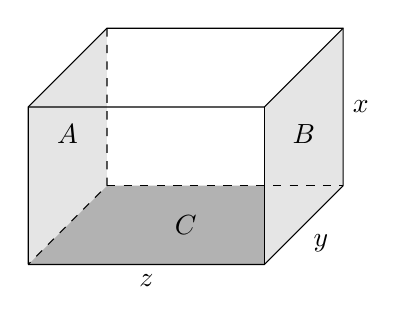
\begin{tikzpicture}
            \fill[black!30] (0, 0) -- (3, 0) -- (3, 1) -- (1, 1) -- cycle;
            \fill[black!10] (0, 0) -- (1, 1) -- (1, 3) -- (0, 2) -- cycle;
            \fill[black!10] (3, 0) -- (4, 1) -- (4, 3) -- (3, 2) -- cycle;

            \draw (0, 0) -- (3, 0) -- (4, 1) -- (4, 3) -- (1, 3) -- (0, 2) -- (0, 0);
            \draw (0, 2) -- (3, 2) -- (4, 3);
            \draw (3, 2) -- (3, 0);
            \draw[dashed] (1, 3) -- (1, 1) -- (0, 0);
            \draw[dashed] (1, 1) -- (4, 1);
            
            \node[anchor=west] at (4, 2) {$x$};
            \node[anchor=north west] at (3.5, 0.5) {$y$};
            \node[anchor=north] at (1.5, 0) {$z$};

            \node at (2, 0.5) {$C$};
            \node at (3.5, 1.65) {$B$};
            \node at (0.5, 1.65) {$A$};
        \end{tikzpicture}
    \end{center}

    \begin{enumerate}
        \item Find the dimensions of the box such that $S$ is minimum.
        \item By differentiating $S$ with respect to $t$, find the rate of change of $S$ if $x$ and $y$ are increasing at a constant rate of $1/2$ units per second and $-1/3$ units per second respectively when $x = 1$, $y = 3$ and $z = 1$.
    \end{enumerate}
\end{problem}
\begin{solution}
    \begin{ppart}
        The surface area $S$ is given by \[S = 4xy + 3yz + 2zx.\] Noting that $xyz = 3$, we get \[S = \frac{12}{z} + \frac{9}x + \frac{6}{y}.\] By the AM-GM inequality, we see that \[S \geq 3 \sqrt[3]{\frac{12 \cdot 9 \cdot 6}{zxy}} = 18.\] Observe that \[\frac{12}{z} = \frac{9}{x} = \frac{6}{y} \iff 3 = xyz = x\bp{\frac{6}{9}x}\bp{\frac{12}{9} x} = \frac89 x^3 \iff x = \frac32,\] so the minimum surface area of 18 units$^2$ is achieved when $x = 3/2$ units, $y = 1$ units, and $z = 2$ units.
    \end{ppart}
    \begin{ppart}
        We have $\derx{x}{t} = 1/2$ and $\derx{y}{t} = -1/3$. We also have \[S = 4xy + \frac9x + \frac6y,\] so
        \begin{align*}
            \der{S}{t} &= \pder{S}{x} \der{x}{t} + \pder{S}{y} \der{y}{t}\\
            &= \frac12\bp{4y - \frac9{x^2}} - \frac13 \bp{4x - \frac6{y^2}}\\
            &= \frac7{18}.
        \end{align*}
        Hence, $S$ is increasing at a rate of $7/18$ units$^2$ per second.
    \end{ppart}
\end{solution}

\clearpage
\begin{problem}
    \begin{enumerate}
        \item Let $M : \RR^3 \to \RR^2$ be defined by \[M \cveciii{a}{b}{c} = \cvecii{a + b}{c}.\] Show that $M$ is a linear transformation.
        \item Let $T : \RR^3 \to \RR^3$ be a linear transformation. Let $T^m = \underbrace{T \circ T \circ \dots \circ T}_{\text{$m$ times}}$ denote the composition of $T$ with itself $m$ times. It is known that \[N_{k-1} \subseteq N_k \tag{$\ast$}\] for all positive integers $k$, where $N_m$ is the null space of $T^m$.
        \begin{enumerate}
            \item Use ($\ast$) to prove that if the null space of $T^{k-1}$ is equal to the null space of $T^k$ for some positive integer $k$, then the null space of $T^k$ is equal to the null space of $T^{k+1}$.
            \item Given that $m$ is the smallest positive integer such that $T^m(\vec w) = \vec 0$ for all $\vec w \in \RR^3$ and the nullity of $T$ is non-zero, explain why $m \leq 3$.
        \end{enumerate}
    \end{enumerate}
\end{problem}
\begin{solution}
    \begin{ppart}
        Let $\vec x = \cveciiix{a_x}{b_x}{c_x}, \vec y = \cveciiix{a_y}{b_y}{c_y} \in \RR^3$ and $k \in \RR$. Then
        \begin{align*}
            M(\vec x + k \vec y) &= M\cveciii{a_x + ka_y}{b_x + kb_y}{c_x + kc_y}\\
            &= \cvecii{a_x + ka_y + b_x + kb_y}{c_x + c_y}\\
            &= \cvecii{a_x + b_x}{c_x} + k\cvecii{a_y + b_y}{c_y}\\
            &= M(\vec x) + k M(\vec y).
        \end{align*}
        Thus, $M$ is a linear transformation.
    \end{ppart}
    \begin{ppart}
        \begin{psubpart}
            Take an arbitrary $\vec x \in N_{k+1}$. By definition, we have $T^{k+1}(\vec x) = \vec 0$. We can rewrite this as $T^k(T(\vec x)) = \vec 0$, so $T(\vec x) \in N_k$. But $N_k = N_{k-1}$, so $T(\vec x) = \vec 0$ hence $T^{k-1}(T(\vec x)) = \vec 0$. Rewriting, we have $T^k(\vec x) = \vec 0$, so $\vec x \in N_k$. Thus, $N_{k+1} \subseteq N_k$. Since $N_k \subseteq N_{k+1}$ by ($\ast$), it follows that $N_k = N_{k+1}$.
        \end{psubpart}
        \begin{psubpart}
            Suppose for a contradiction that there exists some $k \leq m$ such that $N_{k-1} = N_k$. By (b)(i), we will have $N_{k-1} = N_k = N_{k+1} = \dots = N_m = \RR^3$, so $T^{k-1}(\vec w) = \vec 0$ for all $\vec w \in \RR^3$, contradicting the minimality of $m$. Thus, for all $k \leq m$, we have $N_{k-1} \subset N_k$. It follows that \[0 < \dim N_1 < \dim N_2 < \dots < \dim N_m = \dim \RR^3 = 3,\] where the first inequality follows from the fact that the nullity of $T$ is non-zero. It is thus clear that $m \leq 3$.
        \end{psubpart}
    \end{ppart}
\end{solution}

\clearpage
\begin{problem}
    An oncologist is studying the growth of a tumour in one of her patients. The oncologist believes the size of the tumour, $P$ (in millimetres), at the time $t$ months after it was first diagnosed can be modelled by the differential equation \[\der{P}{t} = kP \bp{1 - \frac{P}{N}},\] where $k$ and $N$ are constants.

    \begin{enumerate}
        \item State, in context, the significance of the constants $k$ and $N$ in the model.
        \item Given that $P_0$ is the initial size of the tumour when it was first diagnosed, show that the size of the tumour $P$ after $t$ months is \[P = \frac{P_0 N}{P_0 + (N - P_0) \e^{-kt}}.\]
        \item The oncologist needs to analyse the tumour's growth pattern to determine the best course of action for treatment. She found that the tumour size has grown to 5 times its original size at the end of 2 months. Assuming that $N = 25 P_0$, find the exact value of $k$.
    \end{enumerate}

    After analysing the tumour growth, the oncologist decides to start her patient on chemotherapy. The growth rate of the size of tumour now follows the differential equation \[\der{P}{t} = kP \bp{1 - \frac{P}{N}} - HP,\] where $H$, the therapy induced death rate, is a positive constant.

    \begin{enumerate}
        \setcounter{enumi}{3}
        \item Given that the tumour was detected early, find the range of values of $H$, in terms of $k$, for the tumour to shrink in size and eventually be eradicated.
    \end{enumerate}
\end{problem}
\begin{solution}
    \begin{ppart}
        $N$ is the maximum size of the tumour in millimetres. $k$ controls the rate of growth of the tumour.
    \end{ppart}
    \begin{ppart}
        Rewriting the given differential equation, we have \[\frac1{(N/2)^2 - (P - N/2)^2} \der{P}{t} = \frac{k}{N}.\] Integrating both sides with respect to $t$, we get \[\int \frac1{(N/2)^2 - (P - N/2)^2} \d P = \frac{k}{N} \int \d t.\] Thus, \[\frac1{N} \ln{\frac{P}{N-P}} = \frac{k}{N} t + C_1,\] where we dropped the modulus since $0 < P < N$ by (a). This simplifies to \[P = \frac{C_2 N}{C_2 + \e^{-kt}},\] where $C_2 = \e^{NC_1}$. When $t = 0$, we have $P = P_0$, thus \[C_2 = \frac{P_0}{N-P_0}.\] Hence, $P$ is given by \[P = \frac{P_0 N}{P_0 + (N - P_0) \e^{-kt}}.\]
    \end{ppart}
    \begin{ppart}
        When $t = 2$, we have $N = 25P_0$ and $P = 5P_0$. Substituting this into the above expression yields \[5P_0 = \frac{25P_0^2)}{P_0 + 24P_0\e^{-2k}} \implies 5 = \frac{25}{1 + 24\e^{-2k}}.\] This gives $k = \ln{6}/2$.
    \end{ppart}
    \begin{ppart}
        Consider the critical points of $P$. Setting $\derx{P}{t} = 0$, we get \[kP\bp{1 - \frac{P}{N}} - HP = 0\] so $P = 0$ or $P = \frac{N}{k} (k-H)$. In order for the critical point at $P = 0$ to be stable (hence eradicating the tumour), we must have $\frac{N}{k} (k-H) < 0$. Since $N$ and $k$ are positive constants, we must have $H > k$.
    \end{ppart}
\end{solution}

\begin{problem}
    A colony of bacteria is growing on an agar plate. It is estimated that the initial population of bacteria on the plate was 6000 and that the population at the end of the first day was 9000.

    From previous studies, it is known that the increase in bacteria population from day $n$ to day $n+1$ is twice the increase from day $n-1$ to day $n$.

    \begin{enumerate}
        \item \begin{enumerate}
            \item Let $b_n$ denote the population of bacteria at the end of the $n$th day. Find an expression for $b_n$ in terms of $n$.
            \item Deduce the predicted size of the bacteria population at the end of the 6th day.
        \end{enumerate}
    \end{enumerate}

    Another agar plate containing a colony of the same bacteria with same initial population was contaminated with a virus which kills the bacteria while it was trying to grow. The population of bacteria for this plate can be modelled by the recurrence relation \[c_n = \frac{3c_{n-1} - 2 c_{n-2}}{1+k}\] where $0.2 < k < 1$ and $c_n$ denotes the population of bacteria at the end of the $n$th day.

    \begin{enumerate}
        \setcounter{enumi}{1}
        \item Given that the population of the bacteria at the end of the first day was 9000, and that the population of the bacteria was eliminated at the end of the 6th day, find the value of $k$.
    \end{enumerate}
\end{problem}
\begin{solution}
    \begin{ppart}
        \begin{psubpart}
            We are given that \[b_{n+1} - b_n = 2(b_n - b_{n-1}).\] It is clear that the sequence $\bc{b_n - b_{n-1}}$ is in geometric progression with common ratio 2, so \[b_n - b_{n-1} = 2^{n-1} \bp{b_1 - b_0} = 2^{n-1} (9000 - 6000) = 3000 \cdot 2^{n-1}.\] Thus,
            \begin{align*}
                b_n &= b_0 + \sum_{i = 1}^{n} \bp{b_i - b_{i-1}}\\
                &= 6000 + \sum_{i = 1}^n \bp{3000 \cdot 2^{i-1}}\\
                &= 6000 + 3000 \cdot \frac{2^n - 1}{2-1}\\
                &= 3000 \bp{1 + 2^n}.
            \end{align*}
        \end{psubpart}
        \begin{psubpart}
            We have $b_6 = 3000(1 + 2^6) = 195$ thousand.
        \end{psubpart}
    \end{ppart}
    \begin{ppart}
        From the given recurrence relation, we have \[(1+k) c_n - 3c_{n-1} + 2c_{n-2} = 0.\] The characteristic equation is thus \[(1+k)m^2 - 3m + 2 = 0,\] with roots \[m = \frac{3 \pm \sqrt{1-8k}}{2(1+k)}.\] Since $k > 0.2$, we have $1 - 8k < 0$, so \[m = \frac3{2(1+k)} + \frac{\sqrt{8k-1}}{2(1+k)} \i = \sqrt{\frac2{1+k}} \e^{\pm \i \t},\] where $\t = \arctan{\sqrt{8k-1}/3}$. The general solution is thus \[c_n = \bp{\frac2{1+k}}^{n/2} \bp{A \cos n\t + B \sin n\t}.\] From the initial conditions, we see that $A = c_0 = 6000$ so \[9000 = c_1 = \sqrt{\frac2{1+k}} \bp{6000 \cos \t + B \sin \t}.\] Noting that \[\cos \t = \frac{3}{\sqrt{8(1+k)}} \quad \tand \quad \sin \t = \frac{\sqrt{8k-1}}{\sqrt{8(1+k)}},\] we obtain \[B = \frac{18000k}{\sqrt{8k-1}}.\] Since $c_6 = 0$, we get \[\bp{\frac2{1+k}}^3 \bp{6000\cos 6\t + \frac{18000k}{\sqrt{8k-1}} \sin 6\t} = 0 \implies \tan 6\t = -\frac{\sqrt{8k-1}}{3k}.\] Using G.C., the only root in the interval $(0.2, 1)$ is $k = 0.294$.
    \end{ppart}
\end{solution}

\clearpage
\begin{problem}
    A particular machine part in a factory is known to fail over time more rapidly due to ageing. Its reliability is measured in the number of hours of use before it needs to be replaced. The manufacturer of the machine part models its reliability by the random variable $R$ (in hours) with cumulative distributive function \[F(r) = \begin{cases}
        1 - \e^{-(r/3200)^{3.2}}, & r \geq 0,\\
        0, & r < 0.
    \end{cases}\]

    \begin{enumerate}
        \item Find the probability that the machine part will last more than another 1400 hours given that it has lasted more than 2000 hours.
    \end{enumerate}

    The factory owner who purchases large quantities of the machine part from the manufacturer recorded the reliability of a random sample of 210 of these parts over a period of time with the observed frequencies as follows.

    \begin{table}[H]
        \centering
        \begin{tabular}{|c|c|}
        \hline
        \textbf{Reliability, $R$ (hours)} & \textbf{Observed Frequency} \\ \hline\hline
        $R < 2000$ & 53 \\ \hline
        $2000 \leq R < 2500$ & 41 \\ \hline
        $2500 \leq R < 3000$ & $\b$ \\ \hline
        $3000 \leq R < 3500$ & 26 \\ \hline
        $3500 \leq R < 4000$ & $70 - \b$ \\ \hline
        $4000 \leq R < 4500$ & 16 \\ \hline
        $4500 \leq R < 5000$ & 3 \\ \hline
        $R \geq 5000$ & 1 \\ \hline
        \end{tabular}
    \end{table}

    \begin{enumerate}
        \setcounter{enumi}{1}
        \item Given that a chi-square goodness of fit test at the 5\% significance level concluded that the data is not consistent with the manufacturer's model, find the range of values of $\b$.
    \end{enumerate}
\end{problem}
\begin{solution}
    \begin{ppart}
        We have \[\P{R > 3400}{R > 2000} = \frac{\P{R > 3400}}{\P{R > 2000}} = \frac{1 - F(3400)}{1 - F(2000)} = 0.371 \tosf{3}.\]
    \end{ppart}
    \begin{ppart}
        Let \nullhyp: data is consistent with the given model, and \althyp: data is inconsistent with the given model. Under \nullhyp, the expected frequencies are

        \begin{table}[H]
            \centering
            \begin{tabular}{|c|c|c|}
            \hline
            \textbf{Reliability, $R$ (hours)} & \textbf{$E_i$} & \textbf{$O_i$} \\ \hline\hline
            $R < 2000$ & 41.8 & 53 \\ \hline
            $2000 \leq R < 2500$ & 34.8 & 41 \\ \hline
            $2500 \leq R < 3000$ & 40.3 & $\b$ \\ \hline
            $3000 \leq R < 3500$ & 37.7 & 26 \\ \hline
            $3500 \leq R < 4000$ & 28.2 & $70 - \b$ \\ \hline
            $4000 \leq R < 4500$ & 16.5 & 16 \\ \hline
            $4500 \leq R < 5000$ & 7.45 & 3 \\ \hline
            $R \geq 5000$ & 3.24 & 1 \\ \hline
            \end{tabular}
        \end{table}
        Since the last row has expected frequency less than 5, we combine it with the second last row to form the category $R \geq 4500$. Our test statistic is hence $\sum (O_i - E_i)^2/E_i \sim \ChiSq{7-1} = \ChiSq{6}$. From G.C., the critical value is $\c^2 = 12.592$. Since \nullhyp{} is rejected, we have $\sum (O_i - E_i)^2/E_i \geq 12.592$. Thus, \[11.920 + \frac{(\b - 40.3)^2}{40.3} + \frac{(70 - \b - 28.2)^2}{28.2} \geq 12.592.\] This gives $0 \leq \b \leq 37.9$ or $44.4 \leq \b \leq 70$. Since $\b$ is an integer, the range of values of $\b$ is $0 \leq \b \leq 37$ or $45 \leq \b \leq 70$, where $\b \in \ZZ^+$.
    \end{ppart}
\end{solution}

\begin{problem}
    A language learning app is testing whether its new AI pronunciation coach improves users' pronunciation fluency. Twelve users were scored on a scale of 0 to 100 (with each score given to 1 decimal place) before and after using the app for 2 weeks. A higher score indicates better pronunciation fluency.

    \begin{table}[H]
        \centering
        \begin{tabular}{|c|c|c|}
        \hline
        \textbf{User} & \textbf{Before} & \textbf{After} \\ \hline\hline
        1 & 70.0 & 73.2 \\ \hline
        2 & 65.5 & 69.0 \\ \hline
        3 & 75.1 & 72.4 \\ \hline
        4 & 68.0 & 64.3 \\ \hline
        5 & 72.2 & 76.0 \\ \hline
        6 & 69.8 & 72.7 \\ \hline
        7 & 66.4 & 71.9 \\ \hline
        8 & 75.0 & 72.0 \\ \hline
        9 & 67.0 & 66.1 \\ \hline
        10 & 73.0 & 77.6 \\ \hline
        11 & 70.1 & 67.8 \\ \hline
        12 & 64.5 & 70.7 \\ \hline
        \end{tabular}
    \end{table}

    \begin{enumerate}
        \item Explain why a test based on the $t$-distribution might not be suitable in this context.
        \item Carry out a suitable Wilcoxon test, using a 5\% level of significance, to show that there is insufficient evidence to claim that the app is effective in improving users' pronunciation fluency.
        \item It was subsequently discovered that User 11's score after the use of the app was recorded wrongly. With the correct score in place, the Wilcoxon test will now lead to the conclusion that there is sufficient evidence at a 5\% level of significance that the app is effective in improving users' pronunciation fluency. Given that the rank for each user remains unchanged, determine the lowest possible correct score for User 11 after using the app. Explain how you arrive at your answer.
    \end{enumerate}
\end{problem}
\begin{solution}
    \begin{ppart}
        We may not be able to assume that the difference in scores is normally distributed.
    \end{ppart}
    \begin{ppart}
        Let $m$ be the median change in scores. Let \nullhyp: $m = 0$, \althyp: $m > 0$. We take a 5\% significance level. From the data,

        \begin{table}[H]
            \centering
            \begin{tabular}{|c|c|c|c|c|}
            \hline
            \textbf{User} & \textbf{Before} & \textbf{After} & \textbf{Change} & \textbf{Rank} \\ \hline\hline
            1 & 70.0 & 73.2 & \phantom{$-$}3.2 & 6\\ \hline
            2 & 65.5 & 69.0 & \phantom{$-$}3.5 & 7\\ \hline
            3 & 75.1 & 72.4 & $-$2.7 & 3\\ \hline
            4 & 68.0 & 64.3 & $-$3.7 & 8\\ \hline
            5 & 72.2 & 76.0 & \phantom{$-$}3.8 & 9\\ \hline
            6 & 69.8 & 72.7 & \phantom{$-$}2.9 & 4\\ \hline
            7 & 66.4 & 71.9 & \phantom{$-$}5.5 & 11\\ \hline
            8 & 75.0 & 72.0 & $-$3.0 & 5\\ \hline
            9 & 67.0 & 66.1 & $-$0.9 & 1\\ \hline
            10 & 73.0 & 77.6 & \phantom{$-$}4.6 & 10\\ \hline
            11 & 70.1 & 67.8 & $-$2.3 & 2\\ \hline
            12 & 64.5 & 70.7 & \phantom{$-$}6.2 & 12\\ \hline
            \end{tabular}
        \end{table}

        Let $P$ and $Q$ be the sum of the positive and negative ranks, respectively. Let $T$ be the smaller of the two. From the data, we have $p = 59$ and $q = 19$, so $t = 19$. We reject \nullhyp{} if $t \leq 17$. Since $t = 19 > 17$, we do not reject \nullhyp{} and conclude there is insufficient evidence at the 5\% level that the app is effective in improving users' fluency.
    \end{ppart}
    \begin{ppart}
        User 11's difference is now positive. Let his new score be $x$. Since his rank remains the same, we have $0.9 < x - 70.1 < 2.7$, so $71.0 < x < 72.8$. Since all scores are rounded to 1 decimal place, the lowest possible score is $71.1$.
    \end{ppart}
\end{solution}

\begin{problem}
    Mrs Yeo occasionally allows her son to drive her car. After Mrs Yeo drives the car, the amount of petrol in the car is uniformly distributed between 10 litres and 50 litres. After her son drives the car, the amount of petrol in the tank is uniformly distributed between 0 litres and 20 litres. Mrs Yeo is the drive for 80\% of the time and her son is the driver for the remaining 20\% of the time.

    \begin{enumerate}
        \item Mrs Yeo checks the car at home, not knowing who drove it last. Find the probability that there is less than 15 litres of petrol in the tank.
    \end{enumerate}

    Let $T$ be the random variable denoting the amount of petrol in the tank in litres after someone used the car.

    \begin{enumerate}
        \setcounter{enumi}{1}
        \item Find the cumulative distribution function of $T$. Hence or otherwise, find $\E{T}$.
        \item The maximum distance, in km, of the car journey, $D$, depends on $T$ such that \[D = 650 - \frac{3250}{T + 5}.\] Find the probability that the next driver can drive at least 504 km before it runs out of petrol.
    \end{enumerate}
\end{problem}
\begin{solution}
    \begin{ppart}
        Let $X$ and $Y$ be the amount of petrol left (in litres) after Mrs Yeo and her son drives the car, respectively. Then $X \sim \Uni{10}{50}$ and $Y \sim \Uni{0}{20}$. By the last of total probability,
        \begin{align*}
            &\P{\text{less than 15 litres left}}\\
            &\hspace{1em}= \P{X < 15} \P{\text{Mrs Yeo last drove the car}} + \P{Y < 15} \P{\text{Her son last drove the car}}\\
            &\hspace{1em}= \frac{5}{40} (0.8) + \frac{15}{20} (0.2)\\
            &\hspace{1em}= 0.25.
        \end{align*}
    \end{ppart}
    \begin{ppart}
        Note that \[F_X = \begin{cases}
                0, & x < 10,\\
                \frac{x-10}{40}, & 10 \leq x \leq 50,\\
                1, & x > 50,
            \end{cases} \quad \tand \quad F_Y = \begin{cases}
                0, & y < 0,\\
                \frac{y}{20}, & 0 \leq y \leq 20,\\
                1, & y > 20.
            \end{cases}\]
        Thus, by the law of total probability \[F_T = \begin{cases}
            0 , & t < 0,\\
            0 (0.8) + \frac{t}{20} (0.2), & 0 \leq t < 10,\\
            \frac{t-10}{40} (0.8) + \frac{t}{20} (0.2), & 10 \leq t < 20,\\
            \frac{t-10}{40} (0.8) + 1 (0.2), & 20 \leq t \leq 50,\\
            1 , & t > 50,
        \end{cases} = \begin{cases}
            0 , & t < 0,\\
            0.01t, & 0 \leq t < 10,\\
            0.03t - 0.2, & 10 \leq t < 20,\\
            0.02t, & 20 \leq t \leq 50,\\
            1 , & t > 50.
        \end{cases}\]
        Differentiating, we see that the pdf of $T$ is given by \[f_T = \begin{cases}
            0.01, & 0 \leq t < 10,\\
            0.03, & 10 \leq t < 20,\\
            0.02, & 20 \leq t \leq 50,\\
            0, & \ow.
        \end{cases}\]
        Hence, \[\E{T} = \int_{-\infty}^\infty tf_T(t) \d t = \int_0^{10} 0.01t \d t + \int_{10}^{20} 0.03t \d t + \int_{20}^{50} 0.02t \d t = 26.\]
    \end{ppart}
    \begin{ppart}
        We have
        \begin{align*}
            \P{D > 504} &= \P{650 - \frac{3250}{T + 5} > 504} = \P{T \geq \frac{1260}{73}}\\
            &= 1 - F_T\!\bp{\frac{1260}{73}} = 1 - \bs{0.03\bp{\frac{1260}{73}} - 0.2}\\
            &= \frac{249}{365}.
        \end{align*}
    \end{ppart}
\end{solution}

\begin{problem}
    \begin{enumerate}
        \item Let $X$ be a random variable that follows the Poisson distribution with mean $\l$. It is given that \[\sum_{r = 1}^\infty r^2 \P{X = r} = 2.\] Find the value of $\l$.
        \item In a particular boarding school with many students, the students do not stay with their parents. The number of telephone calls home $D$ made by a female student each week has a Poisson distribution with mean 2, whilst the number of telephone calls home $S$ made by a male student each week has a Poisson distribution with mean 1. A male and a female student are chosen randomly.
        \begin{enumerate}
            \item Find the probability that both students make an equal number of calls home not exceeding 2 calls each in a week.
            \item The probability that either of them makes at least a call home within $n$ days is more than $0.8$. Find the least value of $n$.
            \item Find the probability that the female student makes less than 8 calls home but more than the number of calls the male student makes in a randomly chosen week.
            \item Given that, in a particular week, a total of 7 calls were made, find the probability that the difference between the number of calls home made by the female and the male student is more than 3.
        \end{enumerate}
    \end{enumerate}
\end{problem}
\begin{solution}
    \begin{ppart}
        We are given that $\E{X^2} = 2$. Since $\E{X} = \l$, we get \[\l = \Var{X} = \E{X^2} - \E{X}^2 = 2 - \l^2.\] Hence, $\l^2 + \l - 2 = (\l+2)(\l-1) = 0$, so $\l = 1$. Note that we reject $\l = -2$ since $\l > 0$.
    \end{ppart}
    \begin{ppart}
        We are given that $D \sim \Po{2}$ and $S \sim \Po{1}$.

        \begin{psubpart}
            The required probability is \[\sum_{i = 0}^2 \P{D = i} \P{S = i} = 0.199 \tosf{3}.\]
        \end{psubpart}
        \begin{psubpart}
            Note that $D + S \sim \Po{3}$. Let $X_n \sim \Po{3n/7}$. Then \[\P{X_n > 0} > 0.8 \implies \P{X_n = 0} < 0.2.\] So $\e^{-3n/7} < 0.2$, whence $n > 3.76$. Since $n$ is an integer, the least value of $n$ is 4.
        \end{psubpart}
        \begin{psubpart}
            The required probability is \[\P{S < D < 8} = \sum_{i = 0}^6 \P{S < i} \P{i < D < 8} = 0.605 \tosf{3}.\]
        \end{psubpart}
        \begin{psubpart}
            The required probability is
            \begin{align*}
                &\P{\abs{D - S} > 3}{D + S = 7}\\
                &\hspace{1em}= \frac{\P{D + S = 7 \, \tand \, \abs{D - S} > 3}}{\P{D + S = 7}}\\
                &\hspace{1em}= \frac{\P{D = 0} \P{S = 7} + \P{D = 1}\P{S = 6} + \P{D = 6} \P{S = 1} + \P{D = 7} \P{S = 0}}{\P{D + S = 7}}\\
                &\hspace{1em}= 0.270 \tosf{3}.
            \end{align*}
        \end{psubpart}
    \end{ppart}
\end{solution}

\begin{problem}
    Japple engages a mobile phone manufacturer to make the batteries for its new range of j-phones. One of the requirements is that a new battery should have a mean battery life of 10 hours under regular usage before needing to be recharged.

    To find out if the manufacturer has met this requirement, Japple took a random sample of 10 new batteries and recorded the battery life (in hours) under regular usage in their j-phones as follows.

    \begin{table}[H]
        \centering
        \begin{tabular}{|c|c|c|c|c|c|c|c|c|c|}
        \hline
        \textbf{\#1} & 8.47 & \textbf{\#2} & 11.36 & \textbf{\#3} & 10.26 & \textbf{\#4} & 9.59 & \textbf{\#5} & 7.38 \\ \hline
        \textbf{\#6} & 7.38 & \textbf{\#7} & 6.89 & \textbf{\#8} & 10.93 & \textbf{\#9} & 9.61 & \textbf{\#10} & 10.14 \\ \hline
        \end{tabular}
    \end{table}

    \begin{enumerate}
        \item Stating any assumption(s) required, find a 95\% confidence interval for the mean battery life, leaving your answers to 3 decimal places. Working should be shown.
    \end{enumerate}

    Japple decides to take another random sample of 8 new batteries and repeat the test. For this second sample, a 95\% confidence interval works out to be $(9.015, 9.985)$ (in hours).

    \begin{enumerate}
        \setcounter{enumi}{1}
        \item With the same assumption as in (a), calculate a 95\% confidence interval for all 18 batteries in the 2 samples, leaving your answers to 3 decimal places.
        \item Deduce the conclusion of a hypothesis test for the combined sample, at a 5\% level of significance, on whether the mean battery life is 10 hours.
    \end{enumerate}

    Another requirement of the new batteries is that they must have no difference in their battery life within 50 cycles of full charging. Japple takes the first sample of 10 batteries, subjected them to 50 cycles of full charging and then recorded their battery life (in hours) after the 50th charge as follows:

    \begin{table}[H]
        \centering
        \begin{tabular}{|c|c|c|c|c|c|c|c|c|c|}
        \hline
        \textbf{\#1} & 8.70 & \textbf{\#2} & 11.30 & \textbf{\#3} & 10.22 & \textbf{\#4} & 9.61 & \textbf{\#5} & 7.70 \\ \hline
        \textbf{\#6} & 8.10 & \textbf{\#7} & 7.86 & \textbf{\#8} & 10.70 & \textbf{\#9} & 9.90 & \textbf{\#10} & 9.98 \\ \hline
        \end{tabular}
    \end{table}

    \begin{enumerate}
        \setcounter{enumi}{3}
        \item Assuming that the difference in battery lives before and after the 50 cycles of full charging of a j-phone is normally distributed, carry out a suitable test at a 3\% level of significance and state your conclusion clearly.
    \end{enumerate}
\end{problem}
\begin{solution}
    \begin{ppart}
        Assume that the battery life of a new battery has a normal distribution.

        Let $X$ be the battery life of a j-phone (in hours). Then $X \sim \Normal{\m}{\s^2}$. Let $A$ denote the first sample of 10 batteries. Since $n = 10$ is small, \[\frac{\ol{X}_A - \ol{x}_A}{S_A / \sqrt{10}} \sim \StudentT{10-1}.\] From the given data, we have $\ol{x}_A = 9.201$ and $s_A = 1.5804$. Using G.C., a 95\% confidence interval for $\m$ is \[\bp{\ol{x}_A - t_{0.975} \frac{s_A}{\sqrt{10}}, \, \ol{x}_A + t_{0.975} \frac{s_A}{\sqrt{10}}} = (8.070, 10.332).\]
    \end{ppart}
    \begin{ppart}
        Let $B$ denote the second sample of 8 batteries. Since $n = 8$ is small, \[\frac{\ol{X}_B - \ol{x}_B}{S_B / \sqrt{8}} \sim \StudentT{8-1}.\] Thus, the 95\% confidence interval for the second sample is \[\bp{\ol{x}_B - t_{0.975} \frac{s_B}{\sqrt{8}}, \, \ol{x}_B + t_{0.975} \frac{s_A}{\sqrt{8}}} = (9.015, 9.985).\] This gives the system of equations \[\ol{x}_B - 2.36462 \frac{s_B}{\sqrt{8}} = 9.015, \quad \tand \quad \ol{x}_B + 2.36462 \frac{s_B}{\sqrt{8}} = 9.985.\] Solving, we get $\ol{x}_B = 9.5$ and $s_B = 0.58013$. Thus, \[s_B^2 = \frac1{8-1} \bp{\sum x_B^2 - \frac{9.5(8)^2}{8}} = 0.58013^2 \implies \sum x_B^2 = 724.35585.\] Additionally, \[\ol{x}_{A + B} = \frac{9.201(10) + 9.5(8)}{10 + 8} = 9.33389.\] Hence, \[s^2_{A+B} = \frac1{18-1} \bs{\bp{869.0637 + 724.35585} - \frac{(92.01 + 9.5(8))^2}{18}} = 1.48429.\] Since $n = 18$ is small, \[\frac{\ol{X}_{A+B} - \ol{x}_{A+B}}{S_{A+B} / \sqrt{18}} \sim \StudentT{18-1}.\] A 95\% confidence interval for the two samples combined is thus \[\bp{9.33389 - 2.10982 \sqrt{\frac{1.48429}{18}}, \, 9.33389 + 2.10982 \sqrt{\frac{1.48429}{18}}} = (8.728, 9.940).\]
    \end{ppart}
    \begin{ppart}
        Since 10 hours is not within the 95\% confidence interval for the mean, we can conclude that there is sufficient evidence at the 5\% level of significance that the mean is not 10 hours.
    \end{ppart}
    \begin{ppart}
        Let $D$ be the difference between the battery life before and after 50 cycles of full charging and $\m_D$ be the mean of the difference. Let \nullhyp: $\m_D = 0$ and \althyp: $\m_D \neq 0$. We take a 3\% level of significance. Under \nullhyp, the test statistic is \[T = \frac{\ol{D}}{S_D / \sqrt{10}} \sim \StudentT{10-1}.\] From the data, we have $\ol{d} = 0.206$ and $s = 0.389$. From G.C., the $p$-value is $0.128 > 0.03$. Thus, we do not reject \nullhyp{} and conclude that there is insufficient evidence at the 3\% significance level to claim that there is a difference in the battery life before and after the 50 cycles of full charging.
    \end{ppart}
\end{solution}